\documentclass[10pt,openright,twoside,french]{book}

\input philippe2013
\input philippe2013_cours
\input philippe2013_sections
\input philippe2013_chapitre

\usepackage{docmute}

\begin{document}
\renewcommand\MaCouleur{Melon!150}

%___________________________
%===    Page de garde
%------------------------------------------------------

\frontmatter

\titlepage{
\begin{center}
{\Large\bfseries\color{\MaCouleur} Philippe \bsc{De Sousa}}

\vspace*{\stretch{1}}

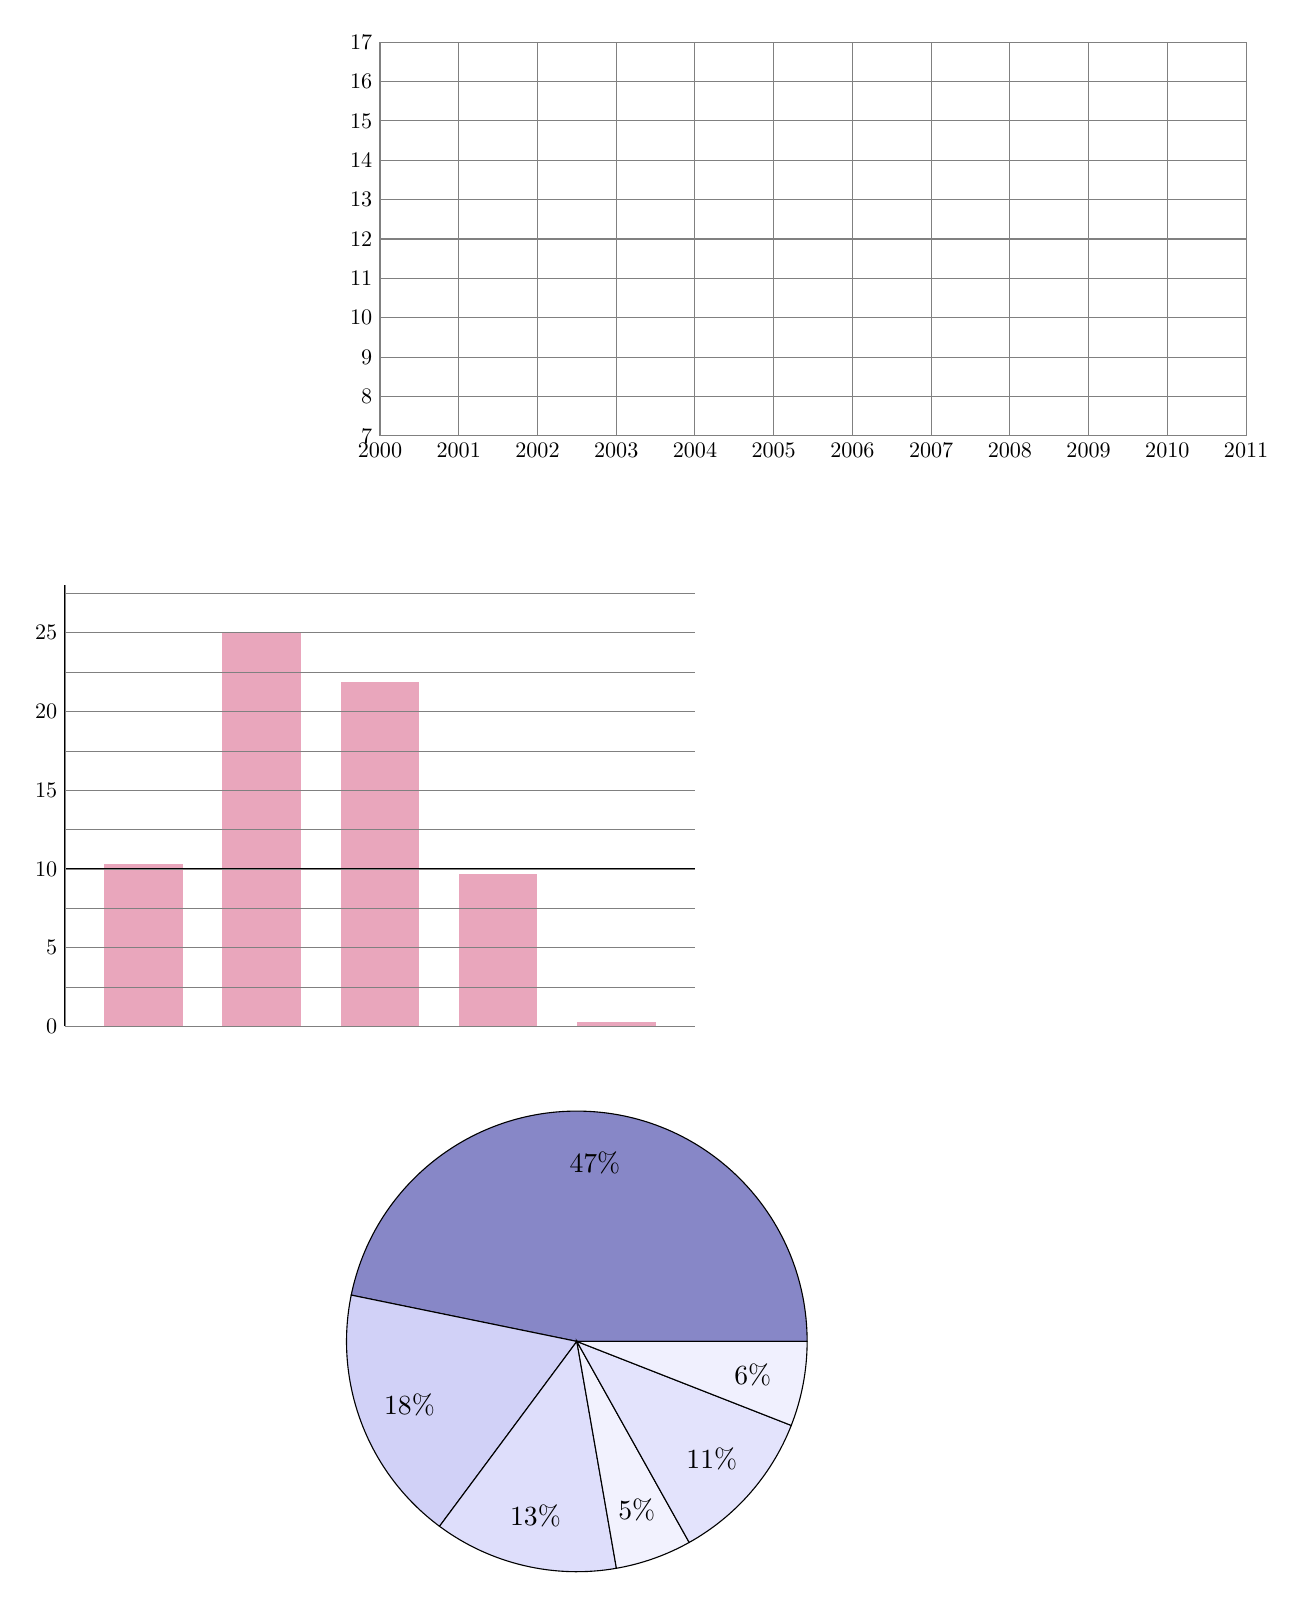
\begin{tikzpicture}
\begin{scope}[xscale=1,yscale=0.2,xshift=-1cm]
\newcommand{\Conso}{(1,10.3)(2.5,25)(4,21.9)(5.5,9.7)(7,0.3)}
\draw[line width=10mm,color=purple!35] plot[ycomb] coordinates {\Conso};
\draw (0,0) grid[xstep=9,ystep=5] (8,28);
\draw[gray,very thin] (0,0) grid[xstep=9,ystep=2.5] (8,28);
\foreach \y in {0,5,...,25} \draw (0,\y) node[left,scale=0.8]{\y};
\end{scope}

\begin{scope}[xshift=3cm,yshift=4cm,yscale=0.5]
\draw[color=OliveGreen,line width=1.5pt] plot[mark=triangle,mark size=3pt] file {Titre1.txt};
\draw[color=blue,line width=1.5pt] plot[mark=diamond,mark size=3pt] file {Titre2.txt};
\draw[thin,gray] (0,7) grid (11,17);
\foreach \y in {7,8,...,17} \draw (0,\y) node[left,scale=0.8]{\y};
\foreach \x in {2000,2001,...,2011} \draw (\x-2000,7) node [below,scale=0.8] {\x};
\end{scope}

\begin{scope}[xshift=5.5cm,yshift=-4cm,scale=0.65]
%\draw[fill=black!47!blue!47] (0,0)--(0:4.5)arc(0:168.4:4.5)--cycle;
%\draw (84:4) node {47\%};
%\draw (84:5.6) node {\bsc{tva}};
\foreach \a/\b/\p/\c in
{
0/168.4/47/\bsc{tva},
168.4/233.4/18/Revenus,
233.4/279.9/13/Sociétés,
279.9/299.2/5/\bsc{tipp},
299.2/338.6/11/{\scriptsize Recettes fiscales},
338.6/360/6/{\scriptsize Recettes}
}{
\draw[fill=black!\p!blue!\p]
(0,0) -- (\a:4.5) arc (\a:\b:4.5) -- cycle;
\draw ({(\a+\b)/2}:3.5) node {\p\%};
}
\end{scope}
\end{tikzpicture}

\begin{tikzpicture}[remember picture,overlay]
\begin{scope}
\node [rotate=45,scale=10,text opacity=0.2]
at (current page.center) {\color{\MaCouleur} Mathématiques};
\end{scope}
\begin{scope}[xshift=5.5cm,yshift=8cm]
\draw[\MaCouleur] (0,0) node[scale=8] {\premiere};
\draw[\MaCouleur] (-0.2,-0.15) node[below,scale=6] {\stmg};
\end{scope}
\end{tikzpicture}

\vspace*{\stretch{1}}

D'après le programme $\NP{2012}$
\end{center}
}

\pieddepage{}{}{}
\entete{}{}{}

\tableofcontents

\mainmatter

\entete{}{\color{\MaCouleur} \textbullet~\leftmark~\textbullet}{}
\pieddepage{}{%
\begin{tikzpicture}[scale=0.65]
\shadedraw [top color=white, bottom color=\MaCouleur, draw=\MaCouleur]
[l-system={Sierpinski triangle, step=1pt, angle=60, axiom=F, order=6.5}]
lindenmayer system -- cycle;
\draw (30:0.65cm) node {\bfseries\textcolor{black}{\thepage}};
\end{tikzpicture}%
}{}
%\pieddepage{}{\color{\MaCouleur}$\stackrel{***}{\thepage}$}{}

%------ Chapitre 01
    \renewcommand\PartProgramme{Info. chiffrée}
    \documentclass[10pt,openright,twoside,french]{book}

\input philippe2013
\input philippe2013_cours
\input philippe2013_sections
\input philippe2013_chapitre
\renewcommand\PartProgramme{Info. chiffrée}
\renewcommand\MaCouleur{Melon!150}

\pieddepage{}{%
\begin{tikzpicture}[scale=0.65]
\shadedraw [top color=white, bottom color=\MaCouleur, draw=\MaCouleur]
[l-system={Sierpinski triangle, step=1pt, angle=60, axiom=F, order=6.5}]
lindenmayer system -- cycle;
\draw (30:0.65cm) node {\bfseries\textcolor{black}{\thepage}};
\end{tikzpicture}%
}{}

\begin{document}

\chapter{\'Evolutions}\label{ch_evolution}

\section{Variations}
On considère une quantité ayant une valeur $y_1$, exprimée dans une unité de mesure. Cette quantité est modifiée et on lui affecte une nouvelle valeur $y_2$, exprimée dans la même unité de mesure.\par
Il y a donc une variation entre $y_1$ et $y_2$.

\subsection{Variation absolue}
\begin{Defi}
    La \ipt{variation absolue} est définie par $y_2 - y_1$.\par
    Si ce nombre est positif, on parlera d'une \textbf{hausse} ou d'une \textbf{augmentation}. Sinon, on parlera d'une \textbf{baisse} ou d'une \textbf{diminution}.
\end{Defi}

\begin{Rmq}
    La variation absolue est exprimée dans la même unité de mesure que la quantité.
\end{Rmq}

\begin{Exemple}[s]
    \begin{description}
        \item[En Essonne :] En $\NP{1990}$, l'Essonne comptait $\NP{1084824}$ habitants. En $\NP{2010}$, ont été comptabilisés $\NP{1215340}$ habitants.\par
        La variation absolue est donc égale à : $\NP{1215340} - \NP{1084824} = \NP{130516}$. Cette variation est positive donc la population en Essonne a augmenté de $\NP{130516}$ habitants en $20$ ans.
        \item[En France :] En $\NP{1990}$, la France comptait $\NP{58 040 660}$ habitants. En $\NP{2010}$, ont été comptabilisés $\NP{64 612 940}$ habitants.\par
        La variation absolue est donc égale à : $\NP{64 612 940} - \NP{58 040 660} = \NP{6572280}$. Cette variation est positive donc la population en France a augmenté de $\NP{6572280}$ habitants en $20$ ans.
    \end{description}
\end{Exemple}

\begin{Rmq}
    \'Evidemment, la variation absolue du nombre d'habitants en France est plus importante que celle du nombre d'habitants en Essonne.\par Comment peut-on alors comparer ces deux évolutions ? En Essonne, l'évolution du nombre d'habitant correspond-elle à l'évolution du nombre d'habitants en France ?
\end{Rmq}

\subsection{Variation relative}
\textbf{Bien comprendre le symbole \% :}
Le symbole \% correspond simplement à une écriture simplifiée d'une fraction ayant pour dénominateur $100$.\medskip

\begin{Exemple}[s]
    $7,5\% = \frac{7,5}{100} = 0,075$.\par\medskip
    $\frac{4}{10} = \frac{40}{100} = 40\%$.\par\medskip
    $0,0125 = \frac{1,25}{100} = 1,25\%$.
\end{Exemple}

\begin{Rmq}[s]
    \begin{itemize}
        \item La variation relative est souvent exprimé à l'aide de pourcentage afin de faciliter les comparaisons.
        \item Il est important de comprendre la signification de la variation relative afin d'éviter parfois certains calculs.
    \end{itemize}
\end{Rmq}\medskip

\begin{Exemple}[s]
    \begin{itemize}
        \item Durant les soldes, un article coûte \EUR{$10$}. À la fin des soldes, l'article coûte \EUR{$20$}. Le prix a doublé : $t = 100\%$.\par
        \item Dans une station service, le Sans Plomb 95 coûte \EUR{$1,52$}. Le lendemain, le prix affiché est de \EUR{$1,52$}. Le prix n'a pas changé donc : $t = 0\%$.
        \item Ce matin, il y avait $60$ croissants à la boulangerie. À midi, il en restait $30$. Le nombre de croissants a diminué de moitié donc $t = -50\%$.
    \end{itemize}
\end{Exemple}\medskip

\begin{Rmq}
    Sauf indication contraire, on supposera jusqu'à la fin du cours que $y_1 \neq 0$.
\end{Rmq}\medskip

\begin{Defi}
    La \ipt{variation relative} ou \ipt{taux d'évolution} $t$ est calculée à partir de la formule suivante : \[t = \frac{y_2 - y_1}{y_1}.\]
    Une fois encore, un nombre positif indique une augmentation et un nombre négatif indique une diminution.
\end{Defi}

\begin{Exemple}[s]
    \begin{description}
        \item[En Essonne :] $t = \frac{\NP{1215340} - \NP{1084824}}{\NP{1084824}} = \frac{\NP{130516}}{\NP{1084824}}\approx \NP{0,1203}$.\par\medskip
        Le taux d'évolution est donc environ égal à $\NP{0,1203}$ : la population a augmenté d'environ $12,03\%$.
        \item[En France :] $t = \frac{\NP{64 612 940} - \NP{58 040 660}}{\NP{58 040 660}} = \frac{\NP{6572280}}{\NP{58 040 660}}\approx \NP{0,1132}$.\par\medskip
        Le taux d'évolution est donc environ égal à $\NP{0,1132}$ : la population a augmenté d'environ $11,32\%$.\medskip
        \item[Conclusion :] En Essonne, l'augmentation de population entre $\NP{1990}$ et $\NP{2010}$ a été légèrement plus importante qu'en France.
    \end{description}
\end{Exemple}

\subsection{Lorsque l'on connaît le taux de variation}
\begin{Exemple}
    Un commerçant de meubles a vendu $125$ chaises ce mois-ci. Son contrat stipule qu'il doit augmenter ses ventes d'au moins $3\%$ chaque mois.\par
    Combien doit-il vendre de chaises le mois prochain ?\medskip

    On commence par calculer l'augmentation souhaitée en nombre de chaises :
    \[3\% \text{ de } 125 = 3\% \times 125 = \frac{3}{100} \times 125 = \frac{3 \times 125}{100} = 3,75.\]
    Le commerçant doit vendre $3,75$ chaises au minimum c'est-à-dire $4$ chaises.\par\smallskip
    On calcule le nombre total : $125 + 4 = 129$. Le commerçant doit vendre au moins $129$ chaises le mois prochain.
\end{Exemple}

\begin{Rmq}
    \textbf{Bilan de l'exemple :}\par
    $y_1$ correspond au nombre de chaises ce mois-ci. Donc $y_1 = 125$.\par
    On cherche la valeur $y_2$ sachant que le taux de variation est égal à $t = 3\% = 0,03$.\par\medskip
    Pour trouver $y_2$, on calcule $3\%$ de $y_1$ en faisant $0,03 \times y_1$ puis on ajoute $y_1$. On obtient alors :
    \[y_2 = y_1 + 0,03y_1 = y_1(1 + 0,03) = (1 + 0,03)y_1.\]
\end{Rmq}\clearpage

On applique le raisonnement précédent à un taux de variation quelconque égal à $t$ :\medskip

\begin{Prop}
    Lorsque l'on passe de la valeur $y_1$ à la valeur $y_2$ avec une variation relative égale à $t$, on a :
    \[y_2 = (1 + t) \times y_1.\]
\end{Prop}

\begin{Demo}
    On peut démontrer la propriété précédente en utilisant la démarche de l'exemple.\par
    Utilisons plutôt la définition du taux de variation :
    \[t = \frac{y_2 - y_1}{y_1} \qLRq t \times y_1 = y_2 - y_1 \qLRq t \times y_1 + y_1 = y_2 \qLRq (t + 1)\times y_1 = y_2.\]
\end{Demo}

\begin{Defi}
    Le nombre $1 + t$ est appelé \ipt{c{\oe}fficient multiplicateur} de $y_1$ à $y_2$.\par
    Un \coef supérieur à $1$ traduit une augmentation, inférieur à $1$ une diminution. S'il est égal à $1$, il n'y a pas de variation.
\end{Defi}

\begin{Exemple}
    Dans une usine, le coût de production $c_1$ d'un objet est égal à \EUR{$\NP{2530}$}.\par
    Afin d'augmenter les bénéfices, le gérant décide de diminuer le coût de production de $2\%$. Quel est alors le nouveau de coût de production $c_2$ ?\medskip

    Puisqu'il s'agit d'une diminution, $t = -2\% = -0,02$ donc :
    \[c_2 = (1+t)c_1 = (1 + (-0,02)) \times \NP{2530} = 0,98 \times \NP{2530} = \NP{2479,40} \text{ \euro}.\]
\end{Exemple}

\section{Taux d'évolution successifs}

\begin{Exemple}
    Dans une commune, le maire décide d'augmenter les impôts locaux de $5\%$.\par
    Ses conseillers lui suggèrent \textit{d'y aller en douceur} en augmentant les impôts seulement de $2\%$ la première année puis de $3\%$ la seconde année.\par
    Le maire doit-il suivre l'avis de ses conseillers ?
\end{Exemple}\medskip

Dans l'exemple précédent, la quantité (impôts) augmente de $y_1$ à $y_2$ puis de $y_2$ à $y_3$. On souhaite connaître le taux de variation $t$ de $y_1$ à $y_3$. Par définition, $t = \frac{y_3 - y_1}{y_1}$. Ici, on ne peut pas utiliser cette définition puisque les valeurs $y_1$ et $y_3$ sont inconnues. On a alors la propriété suivante :\medskip

\begin{Prop}
    On considère une quantité qui évolue de $y_1$ à $y_2$ puis de $y_2$ à $y_3$ avec $y_2 \neq 0$.\par
    On appelle $t_1$ le taux d'évolution de $y_1$ à $y_2$, $t_2$ le taux d'évolution de $y_2$ à $y_3$.\par
    Le taux d'évolution global $t$ permettant de passer de $y_1$ à $y_3$ est tel que :\[1+t = (1 + t_1)(1 + t_2).\]
\end{Prop}

\begin{Rmq}
    Les valeurs $t_1$, $t_2$ et $t$ peuvent évidemment être négatives.
\end{Rmq}

\begin{Demo}
    On sait que $y_3 = (1+t_2) \times y_2$ et $y_2 = (1+t_1)\times y_1$. De plus, $y_3 = (1+t)y_1$. Donc :
    \[y_3 = (1+t_2) \times y_2 = \underbrace{(1 + t_2) \times (1 + t_1)}_{= 1 + t} \times y_1.\]
\end{Demo}

\begin{Exemple}
    Calculons la véritable augmentation des impôts prévus par les conseillers :
    \[1 + t = (1+0,02) \times (1+0,03) = \NP{1,0506}.\]
    L'augmentation sera alors de $5,06\%$ au lieu de $5\%$.
\end{Exemple}

\section{Taux d'évolution réciproque}

\begin{Exemple}
    Afin de faire des économies, un patron décide de baisser les salaires de $4\%$.\par
    Le mois suivant, les ouvriers entrent en grève pour retrouver leur ancien salaire. Le patron accepte et décide alors d'augmenter les salaires de $4\%$ pour qu'ils retrouvent leur valeur d'origine.\par
    La grève doit-elle continuer ?
\end{Exemple}

\begin{Prop}
    On considère une quantité de valeur $y_1 \neq 0$ qui passe à la valeur $y_2 \neq 0$ avec un taux égal à $t$.\par
    Afin de passer de $y_2$ à $y_1$, il faut utiliser le coefficient $t'$ tel que : \[1 + t' = \frac{1}{1 + t}.\]
\end{Prop}

\begin{Rmq}
    On rappelle que $t$ et $t'$ peuvent être négatifs. De plus, on a bien $t \neq -100\%$ puisque $y_2 \neq 0$.
\end{Rmq}

\begin{Demo}
    On a les égalités suivantes : $y_2 = (1 + t)y_1$ et $y_1 = (1+t')y_2$ d'où :
    \[\begin{split}
        y_2 = (1 + t)y_1 = (1+t)(1+t')y_2 &\qLRq 1 = (1+ t)(1+t') \quad (\text{puisque }y_2 \neq 0)\\
                                                           &\qLRq 1+t' = \frac{1}{1+t} \quad (\text{puisque } t \neq -1).
    \end{split}\]
\end{Demo}

\begin{Exemple}
    Le taux appliqué par le patron est égal à $(1 - 0,04)(1 + 0,04) =  \NP{0,9984}$ soit $99,84\%$ ce qui signifie qu'au final, les salaires ont baissé de $0,16\%$.\par
    Il faut donc trouver le taux de variation réciproque $t'$ sachant que $t = -0,04$ et que donc $1+t = 0,96$ :
    \[1+t' = \frac{1}{1+t} \qLRq 1+t' = \frac{1}{0,96} \qLRq t' = \frac{1}{0,96} - 1 \approx \NP{1,0417} \quad \text{donc} \quad \pfr{t' \approx 4,17\%}.\]
\end{Exemple}

\end{document}


%------ Chapitre 02
    \renewcommand\PartProgramme{Fonctions}
    \documentclass[10pt,openright,twoside,french]{book}

\input philippe2013
\input philippe2013_cours
\input philippe2013_sections
\input philippe2013_chapitre
\renewcommand\PartProgramme{Fonctions}
\renewcommand\MaCouleur{Melon!150}

\pieddepage{}{%
\begin{tikzpicture}[scale=0.65]
\shadedraw [top color=white, bottom color=\MaCouleur, draw=\MaCouleur]
[l-system={Sierpinski triangle, step=1pt, angle=60, axiom=F, order=6.5}]
lindenmayer system -- cycle;
\draw (30:0.65cm) node {\bfseries\textcolor{black}{\thepage}};
\end{tikzpicture}%
}{}

\setcounter{chapter}{1}

\begin{document}
\chapter{Suites}\label{ch_suite}

\section{Définir une suite}
\begin{Defi}
    Une \ipt{suite numérique} $u$ est une fonction de $\N$ dans $\R$. On note alors :
    \[\begin{array}{rcl}
        u\colon \N & \to & \R \\
        n & \mapsto & u(n) = u_n
    \end{array}\]
\end{Defi}\medskip

\begin{Rmq}
    Le premier terme de la suite sera alors le terme de rang (d'indice) $0$ : $u(0)$. Le suivant est le terme de rang (d'indice) $1$ : $u(1)$. Puis $u(2)$\ldots Dans le cas des suites, on notera plutôt $u_0$, $u_1$, $u_2$\ldots\par
    Pour parler d'une suite, on dira la suite $u$, ou encore la suite $(u_n)_{n \in \N}$.\par
    Pour alléger l'écriture, on pour écrire la suite $(u_n)$ mais il ne faut pas confondre avec le terme de rang $n$ qui se note $u_n$ ou $u(n)$.
\end{Rmq}

\subsection{Suite définie explicitement}

\begin{Defi}
    Une suite $(u_n)_{n\in \N}$ est définie \iptb{explicitement}\index{suite!définie explicitement} lorsque l'on connaît l'expression de $u_n$ en fonction de $n$. On peut donc calculer directement la valeur de $u_n$.
\end{Defi}

\begin{Exemple}[s]
     \begin{enumerate}
        \item On considère la suite $(u_n)$ définie pour tout $n \in \N$ par $u_n = 2n^2 - 3$.\par
        Le terme initial est $u_0 = 2 \times 0^2 - 3 = -3$. Le terme suivant est $u_1 = 2 \times 1^2 - 3 = -1$.\par
        $u_{10} = 2 \times 10^2 - 3 = 2 \times 100 - 3 = 197$.
        Le quinzième terme est $u_{14} = 2 \times 14^2 - 3 = 389$.
        \item On considère la suite $(v_n)$ définie pour tout $n \in \N^*$ par $v_n = \frac1n$.\par
        Le terme initial est $v_1 = \frac 1 1 = 1$. Le $15$\ieme terme est $v_{15} = \frac{1}{15}$.
     \end{enumerate}
\end{Exemple}

\subsection{Suite définie par récurrence}

\begin{Defi}
    Une suite $(u_n)_{n\in \N}$ est définie par \iptb{récurrence} \index{suite!définie par récurrence} lorsque l'on connaît l'expression de $u_n$ en fonction de $u_{n-1}$. Pour calculer un terme d'une suite, il faut donc connaître le précédent. Pour cela, le terme initial est généralement donné avec la définition de la suite.
\end{Defi}

\begin{Exemple}
    On considère la suite $u_n$ définie par :
    $\left\{
    \begin{array}{l}
        u_0 = \frac 13\\
        u_{n +1} = \frac 34 u_n - 1 \quad \text{pour tout $n\in \N^*$}
    \end{array}
    \right.$\par\medskip
    On a alors $u_0 = \frac 13$, $u_1 = \frac 3 4 \times u_0 - 1 = \frac34 \times \frac 13 - 1 = \frac 14 - 1 = -\frac34$.\par
    Puis $u_2 = \frac 3 4 \times u_1 - 1 = \frac34 \times \left(-\frac 34\right) - 1 = -\frac{9}{16} - 1 = -\frac{25}{16}$
\end{Exemple}

\begin{Rmq}
    Dans tous les cas, l'utilisation d'un tableur ou d'une calculatrice peut s'avérer très utile pour calculer rapidement les premiers termes d'une suite ainsi que pour les représenter graphiquement.
\end{Rmq}

\section{Suites particulières}
\subsection{Suite arithmétique}

\begin{Defi}
    Une suite $(u_n)_{n\in \N}$ est dite \iptb{arithmétique} \index{suite!arithmétique} lorsqu'il existe un nombre réel $r$ tel que, pour tout $n \in \N$, $u_{n+1} = u_n + r$.\par
    Le réel $r$ est appelé la \ipt{raison} de la suite $(u_n)$
\end{Defi}\medskip

\begin{Exemple}
    Des parents ouvrent un compte en banque pour leur enfant. Lors de l'ouverture, ils  versent \EUR{$50$} puis, au début de chaque mois, ils rajoutent \EUR{$100$}.\par
    On définit alors une suite $(c_n)_{n\in\N}$ où le terme $n$ de la suite correspond au montant présent sur le compte $n$ mois après son ouverture.\par
    On a donc $c_0 = 50$ et, pour tout $n \in \N^*$, $c_{n+1} = c_n + 100$.\par
    La suite $(c_n)$ est donc une suite arithmétique.

    \begin{center}
    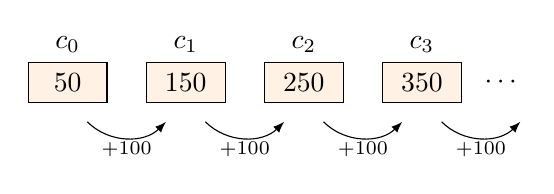
\begin{tikzpicture}[>=latex]
        \draw[fill=orange!10] (0,0) rectangle ++(1,0.5) node[midway] {\EUR{$50$}};
            \draw (0.5,0.5) node[above] {$c_0$};
        \draw[fill=orange!10] (1.5,0) rectangle ++(1,0.5) node[midway] {\EUR{$150$}};
            \draw (2,0.5) node[above] {$c_1$};
        \draw[fill=orange!10] (3,0) rectangle ++(1,0.5) node[midway] {\EUR{$250$}};
            \draw (3.5,0.5) node[above] {$c_2$};
        \draw[fill=orange!10] (4.5,0) rectangle ++(1,0.5) node[midway] {\EUR{$350$}};
            \draw (5,0.5) node[above] {$c_3$};
        \draw (6,0.25) node {$\cdots$};
        %
        \draw[->] (0.75,-0.25) to[bend right=45] ++(1,0); \draw (1.25,-0.6) node {\scriptsize\EUR{$+100$}};
        \draw[->] (2.25,-0.25) to[bend right=45] ++(1,0); \draw (2.75,-0.6) node {\scriptsize\EUR{$+100$}};
        \draw[->] (3.75,-0.25) to[bend right=45] ++(1,0); \draw (4.25,-0.6) node {\scriptsize\EUR{$+100$}};
        \draw[->] (5.25,-0.25) to[bend right=45] ++(1,0); \draw (5.75,-0.6) node {\scriptsize\EUR{$+100$}};
    \end{tikzpicture}
\end{center}
\end{Exemple}\medskip

\begin{Rmq}
    Considérons une suite arithmétique $(u_n)_{n \in \N}$, de raison $r$ et essayons de déterminer une définition explicite de cette suite. Pour tout $n \in \N^*$,
    \[u_{n} = u_{n-1} + r = u_{n-2} + r + r = u_{n-3} + r + r + r = \ldots = u_0 + r + \cdots + r = u_0 + n \times r\]
    On rappelle que $u_0$ et $r$ sont fixés et que le nombre $n$ est la variable. Donc, en employant les notations des fonctions, on obtient :
    \[u(n) = r \times n + u_0.\]
    Non seulement on a défini $(u_n)$ explicitement mais de plus, on constate qu'une suite arithmétique est une fonction affine (définie sur $\N$ uniquement) dont le \coef directeur est la raison $r$ et l'ordonnée à l'origine est $u_0$. On en déduit les résultats suivants :
\end{Rmq}\medskip

\begin{Prop}
    Une suite arithmétique est représentée graphiquement par des points alignés.
\end{Prop}\medskip

\begin{Thm}
    Une suite arithmétique de raison $r$ est :
    \begin{itemize}
        \item croissante si $r > 0$ ;
        \item décroissante si $r < 0$ ;
        \item constante si $r = 0$.
    \end{itemize}
\end{Thm}

\subsection{Suite géométrique}

\begin{Defi}
    Une suite $(u_n)_{n\in \N}$ est dite \iptb{géométrique} \index{suite!géométrique} lorsqu'il existe un nombre réel $q$ \textbf{non nul} tel que, pour tout $n \in \N$, $u_{n+1} = u_n \times q$.\par
    Le réel $q$ est appelé la \ipt{raison} de la suite $(u_n)$
\end{Defi}\medskip

\begin{Exemple}
    Un professeur décide de faire copier des lignes à chaque élève qui parlera sans autorisation. Le premier copiera $10$ lignes, le suivant $2$ fois plus, et ainsi de suite en multipliant le nombre de lignes par $2$ à chaque fois.\par
    On définit alors une suite $(\ell_n)_{n\in\N^*}$ où le terme $n$ de la suite correspond au nombre de ligne copiée par le $n$\ieme élève.\par
    On a donc $\ell_1 = 10$ et, pour tout $n \in \N^*$, $\ell_{n+1} = \ell_n \times 2$.\par
    La suite $(\ell_n)$ est donc une suite géométrique.

    \begin{center}
    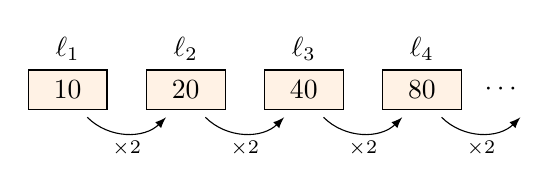
\begin{tikzpicture}[>=latex]
        \draw[fill=orange!10] (0,0) rectangle ++(1,0.5) node[midway] {$10$};
            \draw (0.5,0.5) node[above] {$\ell_1$};
        \draw[fill=orange!10] (1.5,0) rectangle ++(1,0.5) node[midway] {$20$};
            \draw (2,0.5) node[above] {$\ell_2$};
        \draw[fill=orange!10] (3,0) rectangle ++(1,0.5) node[midway] {$40$};
            \draw (3.5,0.5) node[above] {$\ell_3$};
        \draw[fill=orange!10] (4.5,0) rectangle ++(1,0.5) node[midway] {$80$};
            \draw (5,0.5) node[above] {$\ell_4$};
        \draw (6,0.25) node {$\cdots$};
        %
        \draw[->] (0.75,-0.1) to[bend right=45] ++(1,0); \draw (1.25,-0.5) node {\scriptsize$\times 2$};
        \draw[->] (2.25,-0.1) to[bend right=45] ++(1,0); \draw (2.75,-0.5) node {\scriptsize$\times 2$};
        \draw[->] (3.75,-0.1) to[bend right=45] ++(1,0); \draw (4.25,-0.5) node {\scriptsize$\times 2$};
        \draw[->] (5.25,-0.1) to[bend right=45] ++(1,0); \draw (5.75,-0.5) node {\scriptsize$\times 2$};
    \end{tikzpicture}
\end{center}
\end{Exemple}\medskip

\begin{Rmq}
    Considérons une suite géométrique $(v_n)_{n \in \N}$, de raison $q$ et essayons de déterminer une définition explicite de cette suite. Pour tout $n \in \N^*$,
    \[v_{n} = v_{n-1} \times q = v_{n-2} \times q \times q = v_{n-3} \times q \times q \times q = \ldots = v_0 \times q \times \cdots \times q = v_0 \times q^n\]
\end{Rmq}\medskip

\begin{Thm}
    On considère une suite $(u_n)_{n\in\N}$ telle que, pour tout $n \in \N, u_n > 0$.
    On suppose que $(u_n)$ est une suite géométrique de raison $q > 0$. Alors, $(u_n)$ est :
    \begin{itemize}
        \item croissante si $q > 1$ ;
        \item décroissante si $q < 1$ ;
        \item constante si $q = 1$.
    \end{itemize}
\end{Thm}

\begin{Demo}
    \begin{itemize}
        \item Lorsque $q = 1$ alors $u_0 = u_1 = u_2 =\ldots$ et la suite $u$ est constante.
        \item Sinon, pour tout $n \in \N$, on a $u_{n+1} = qu_n$. Puisque, pour tout $n \in \N$, $u_n > 0$, on peut alors écrire $\frac{u_{n+1}}{u_n} = q$. Cette fraction est strictement positive puisque c'est le quotient de deux nombres strictement positif.\par
            Depuis le collège, on sait que si $q<1$, cela signifie que le numérateur est inférieur au dénominateur. Donc, pour tout $n \in \N$, $u_{n+1} < u_n$ et la suite est donc décroissante.\par
            Si $q > 1$, cela signifie que le numérateur est supérieur au dénominateur. Donc, pour tout $n \in \N$, $u_{n+1} > u_n$ et la suite est donc croissante.
    \end{itemize}
\end{Demo}

\end{document}


%------ Chapitre 03
    \renewcommand\PartProgramme{Stats/Probas}
    \documentclass[10pt,openright,twoside,french]{book}

\input philippe2013
\input philippe2013_cours
\input philippe2013_sections
\input philippe2013_chapitre
\renewcommand\PartProgramme{Stats/Probas}
\renewcommand\MaCouleur{Melon!150}

\pieddepage{}{%
\begin{tikzpicture}[scale=0.65]
\shadedraw [top color=white, bottom color=\MaCouleur, draw=\MaCouleur]
[l-system={Sierpinski triangle, step=1pt, angle=60, axiom=F, order=6.5}]
lindenmayer system -- cycle;
\draw (30:0.65cm) node {\bfseries\textcolor{black}{\thepage}};
\end{tikzpicture}%
}{}

\setcounter{chapter}{2}

\begin{document}
\chapter{Statistiques descriptives}\label{ch_stats}

\section{Vocabulaire}

Une \textbf{étude statistique} a pour but d'obtenir une information, appelée \textbf{caractère}, sur une population à partir de \textbf{données} recueillies sur un \textbf{échantillon} de cette population.

\begin{Defi}
    Le \iptb{caractère}\index{caractère!les différents types de} étudié peut être :
    \begin{description}
        \item[quantitatif :] les valeurs du caractère s'expriment avec des nombres (ex : températures, pointures, salaires\ldots) ;
        \item[qualitatif :] les valeurs ne s'expriment pas par des nombres (ex : couleurs, type d'essence\ldots) ;
        \item[discret :] les valeurs du caractère sont isolés (ex : notes\ldots) ;
        \item[continu :] les valeurs sont regroupées par classes (ou intervalles de nombre) (par ex : durée, distance parcourue,
    \end{description}
\end{Defi}

\begin{Rmq}
    Dans la suite du cours, on considère que le caractère est quantitatif.
\end{Rmq}

\begin{Defi}
    Lorsque les valeurs d'une série statistique sont regroupés par classe de type $\intervallefo a b$, on appelle \ipt{centre de classe} le nombre défini par $\frac{a + b}{2}$.
\end{Defi}

\section{Indicateurs de position}
\subsection{Moyenne}
\begin{Defi}
On considère une série qui possède des valeurs différentes $x_1, x_2, \ldots, x_p$ chacune affectée de leur effectif. L'effectif total est égal à $N$.\par
On appelle \ipt{moyenne} d'une série le nombre $\overline{m}$ tel que :
\[\overline{m} = \frac{n_1x_1 + n_2x_2 + n_3x_3 + \cdots + n_px_p}{n_1 + n_2 + \cdots + n_p} = \frac{\displaystyle\sum_{i =1}^{p}n_ix_i}{N}.\]
\end{Defi}

\begin{Exemple}
    Un élève souhaite calculer la moyennes de ses notes sur $20$ : $8 \pv 10 \pv 14 \pv 13 \pv 10 \pv 14 \pv 10$.\par\medskip
    $\overline m = \frac{8 + 10 + 14 + 13 + 10 + 14 + 10}{7} = \frac{79}{7} \approx 11,29$.\medskip

    Parfois, les valeurs sont regroupées dans un tableau : \quad
    \begin{tabular}{*{5}{|c}|}
    \hline
        Notes & $8$ & $10$ & $13$ & $14$ \\
    \hline
        Effectifs & $1$ & $3$ & $1$ & $2$ \\
    \hline
    \end{tabular}\par\medskip
    On peut alors utiliser la formule : $\overline m = \frac{1 \times 8 + 3 \times 10 + 1 \times 13 + 2 \times 14}{1 + 3 + 1 + 2} = \frac{79}{7} \approx 11,29.$
\end{Exemple}

\begin{Rmq}[s]
\begin{enumerate}
    \item En règle générale, la moyenne n'est pas une valeur de la série. On peut la considérer comme le \textnormal{point d'équilibre} des valeurs. Par conséquent, la moyenne est sensible aux valeurs extrêmes.\par
        Pour reprendre l'exemple, si la prochaine note du contrôle est très élevée alors la moyenne va augmenter.
    \item Lorsque les valeurs sont regroupés par classe, au lieu d'utiliser les $x_i$, on utilise les centres de classe.
\end{enumerate}
\end{Rmq}

\begin{Exemple}
    Le tableau ci-dessous regroupe le temps de parcours des habitants d'un village entre leur domicile et leur lieu de travail. Le maire cherche à calculer le temps moyen.
    \begin{center}
    \renewcommand\arraystretch{1.5}
        \begin{tabular}{*{7}{|c}|}
            \hline
                Durée en min & $[0 \pv 10[$ & $[10 \pv 20[$ & $[20 \pv 30[$ & $[30 \pv 50[$ & $[50 \pv 70[$ & Total \\
            \hline
                Effectif & $18$ & $35$ & $25$ & $112$ & $80$ & $270$ \\
            \hline
                Centre de classe & $5$ & $15$ & $25$ & $40$ & $60$ & \\
            \hline
        \end{tabular}
    \renewcommand\arraystretch{1}
    \end{center}
    On a donc : $\overline m = \frac{18 \times 5 + 35 \times 15 + 25 \times 25 + 112 \times 40 + 80 \times 60}{270} = \frac{\NP{10520}}{270} \approx 39~min.$
\end{Exemple}

\subsection{Médiane}

\begin{Defi}
    On considère une série statistique dont l'effectif total est égal à $N$. Les valeurs sont rangées dans l'ordre croissant.

    \textbf{Une} \ipt{médiane} $Me$ est un nombre réel qui permet de partager la série statistique en deux séries de même valeur.

    Autrement dit, la moitié ($50\%$) des valeurs de la série est inférieure ou égale à $Me$ et l'autre moitié est supérieure ou égale à $Me$.

\begin{center}
    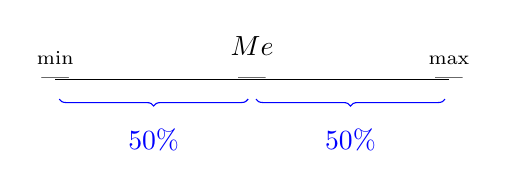
\begin{tikzpicture}
        \draw (0,0)--(5,0) node[midway] {|} node[midway,above=5pt] {$Me$};
        \draw (0,0) node {|} node[above=2pt] {\scriptsize $\min$}; \draw (5,0) node {|} node[above=2pt] {\scriptsize $\max$};
        \draw[color=blue,decorate,decoration={brace,raise=0.25cm}] (2.45,0) -- (0.05,0) node[below=0.5cm,pos=0.5] {$50\%$};
        \draw[color=blue,decorate,decoration={brace,raise=0.25cm}] (4.95,0) -- (2.55,0) node[below=0.5cm,pos=0.5] {$50\%$};
    \end{tikzpicture}
\end{center}
\end{Defi}

\textbf{Méthode de calcul :} Par définition, la médiane dépend de l'effectif de la série :
\begin{itemize}
    \item Si $N$ est impair, alors on calcule $\frac{N + 1}{2}$ et le résultat correspond à la position de la médiane choisie dans la série.
    \item Si $N$ est pair, alors la médiane choisie est égale à la moyenne de la valeur situé à la position $\frac N 2$ et la valeur suivante.
\end{itemize}

\begin{Exemple}
On considère le relevé des températures en janvier et en février dans une ville :
\begin{center}
\renewcommand\arraystretch{1.5}
    \begin{tabular}{*{10}{|c}|}
        \hline
            \multicolumn{10}{|c|}{Janvier}\\
        \hline
            Valeurs & $-3\degres$ & $-2\degres$ & $-1\degres$ & $0\degres$ & $1\degres$ & $2\degres$ & $3\degres$ & $4\degres$ & Total \\
        \hline
            Effectifs & $3$ & $5$ & $8$ & $5$ & $4$ & $3$ & $2$ & $1$ & $31$\\
        \hline
            \multicolumn{10}{|c|}{Février}\\
        \hline
            Valeurs & $-3\degres$ & $-2\degres$ & $-1\degres$ & $0\degres$ & $1\degres$ & $2\degres$ & $3\degres$ & $4\degres$ & Total \\
        \hline
            Effectifs & $1$ & $2$ & $3$ & $3$ & $5$ & $9$ & $3$ & $2$ & $28$\\
            \hline
    \end{tabular}
\renewcommand\arraystretch{1}
\end{center}\medskip

\begin{description}
    \item[En janvier :] $N = 31$ donc $\frac{N+1}{2} = 16$ : une médiane possible est la $16$\ieme valeur donc $Me = -1\degres$. En janvier, il a fait moins de $-1\degres$ la moitié du mois.
    \item[En févier :] $N = 28$ donc $\frac{N}{2} = 14$ : la $14\ieme$ est $1\degres$ et la suivante est égale à $2\degres$. Donc la moyenne des deux est $\frac{1+2}{2} = 1,5$. Une médiane possible est égale à $1,5\degres$ donc durant la moitié du mois, la température a été supérieure à $1,5\degres$.
\end{description}
\end{Exemple}

\begin{Rmq}
    Contrairement à la moyenne, la médiane n'est pas sensible aux valeurs extrêmes. En effet, dans notre exemple, si la dernière température était égale à $20\degres$ au lieu de $4\degres$, la moyenne augmenterait alors que la médiane resterait identique car l'effectif total n'a pas changé.
\end{Rmq}

\subsection{Quartiles}

\begin{Defi}
    On considère une série statistique $S$ dont l'effectif total est égal à $N$. Les valeurs sont rangées dans l'ordre croissant.
    \begin{itemize}
        \item Le \ipt{premier quartile}\index{quartile} $Q_1$ de $S$ est le plus petit élément $a$ de $S$ tel qu'au moins $25\%$ des données soient inférieures ou égales à $a$.
        \item Le \ipt{troisième quartile}\index{quartile} $Q_3$ de $S$ est le plus petit élément $b$ de $S$ tel qu'au moins $75\%$ des données soient inférieures ou égales à $b$.
    \end{itemize}

\begin{center}
    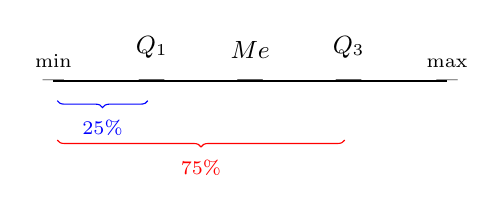
\begin{tikzpicture}
        \begin{small}
        \draw (0,0)--(5,0) node[midway] {|} node[midway,above=5pt] {$Me$} node[pos=0.75,above=5pt] {$Q_3$} node[pos=0.25,above=5pt] {$Q_1$};
        \draw (0,0)--(5,0) node[pos=0.25] {|}; \draw (0,0)--(5,0) node[pos=0.75] {|};
        \end{small}
        \begin{scriptsize}
        \draw (0,0) node {|} node[above=2pt] {$\min$}; \draw (5,0) node {|} node[above=2pt] {$\max$};
        \draw[color=blue,decorate,decoration={brace,raise=0.25cm}] (1.2,0) -- (0.05,0) node[below=0.4cm,pos=0.5] {$25\%$};
        \draw[color=red,decorate,decoration={brace,raise=0.75cm}] (3.7,0) -- (0.05,0) node[below=0.9cm,pos=0.5] {$75\%$};
        \end{scriptsize}
    \end{tikzpicture}
\end{center}
\end{Defi}

\textbf{Méthode de calcul :} Par définition, les quartiles dépendent de l'effectif de la série :
\begin{description}
    \item[Premier quartile :] On arrondit le nombre $\frac{N}{4}$ à l'unité par excès et cela donne la position de $Q_1$ dans la série $S$.
    \item[Troisième quartile :] On arrondit le nombre $3\times\frac{N}{4}$ à l'unité par excès et cela donne la position de $Q_3$ dans la série $S$.
\end{description}

\begin{Exemple}
    On reprend les températures du moins de janvier de l'exemple précédent.
    \begin{description}
        \item[Premier quartile :] $N = 31$ donc $\frac N 4 = 7,75 \approx 8$ donc la $8\ieme$ valeur est $Q_1 = -2\degres$.
        \item[Troisième quartile :] $N = 31$ donc $3\times\frac N 4 = 23,25 \approx 24$ donc la $24\ieme$ valeur donne $Q_3 = 1\degres$.
    \end{description}
    Ainsi, $25\%$ des valeurs sont inférieures ou égales à $-2\degres$ et $75\%$ des valeurs sont inférieures ou égales à $1\degres$. On peut dire aussi que $25\%$ des valeurs sont supérieures ou égales à $1\degres$.
\end{Exemple}

\section{Indicateurs de dispersion}

Dans les classes antérieures, l'\iptb{étendue} était un indicateur de dispersion utilisé dont voici rappelée la définition :

\begin{Defi}
    Dans une série statistique, l'\iptb{étendue}\index{etendue@étendue} est la différence entre la valeur maximale et la valeur minimale.
\end{Defi}

\begin{Rmq}
    Une valeur élevée de l'étendue signifie qu'au moins une des valeurs extrêmes de la série est éloignée de la médiane et le risque de dispersion des valeurs est donc plus important.\par
    Dans l'exemple précédent, l'étendue de la série \textnormal{janvier} était identique à celle de la série \textnormal{février} ce qui montre les besoins d'avoir d'autres indicateurs.\par
    Les quartiles nous permettent d'obtenir d'autres indicateurs de dispersion lié à la médiane.
\end{Rmq}

\subsection{Intervalle et écart interquartile}

\begin{Defi}
    On appelle l'\ipt{intervalle interquartile} l'intervalle $\intervalleff{Q_1}{Q_3}$.\par
    On appelle l'\iptb{écart interquartile}\index{ecart interquartile@écart interquartile} le nombre $Q_3 - Q_1$.
\end{Defi}

\begin{Rmq}
\begin{center}
    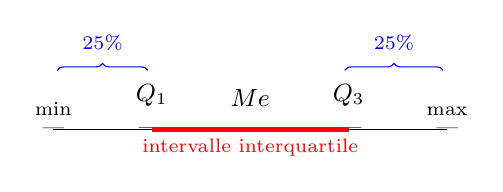
\begin{tikzpicture}
        \begin{small}
        \draw (0,0)--(5,0) node[midway] {|} node[midway,above=5pt] {$Me$} node[pos=0.75,above=5pt] {$Q_3$} node[pos=0.25,above=5pt] {$Q_1$};
        \draw (0,0)--(5,0) node[pos=0.25] {|}; \draw (0,0)--(5,0) node[pos=0.75] {|};
        \end{small}
        \begin{scriptsize}
        \draw (0,0) node {|} node[above=2pt] {$\min$}; \draw (5,0) node {|} node[above=2pt] {$\max$};
        \draw[color=blue,decorate,decoration={brace,raise=0.75cm}] (0.05,0) -- (1.2,0) node[above=0.9cm,pos=0.5] {$25\%$};
        \draw[color=blue,decorate,decoration={brace,raise=0.75cm}] (3.7,0) -- (4.95,0) node[above=0.9cm,pos=0.5] {$25\%$};
        \draw[red,line width=2pt] (1.25,0)--(3.75,0) node[midway,below] {intervalle interquartile};
        \end{scriptsize}
    \end{tikzpicture}
\end{center}

La figure ci-dessus nous permet de comprendre pourquoi l'intervalle interquartile contient $50\%$ de valeurs de la série, c'est-à-dire la moitié. Ainsi, un écart interquartile faible impose que les valeurs soient regroupées proches de la médiane et donc peu dispersée pour la moitié d'entre elles.
\end{Rmq}

Voici maintenant un indicateur de dispersion lié à la moyenne.

\subsection{\'Ecart-type}
\begin{Exemple}
    Voici les notes obtenues par Paul dans quelques matières lors des deux premiers trimestres de l'année.
\begin{description}
        \item[Trimestre 1 :] $7 \pv 8 \pv 11 \pv 12 \pv 13 \pv 13 \pv 13$.
        \item[Trimestre 2 :] $4 \pv 7 \pv 9 \pv 12 \pv 13 \pv 13 \pv 19$.
    \end{description}
    Bien qu'au deuxième trimestre Paul ait obtenu une très bonne note, on remarque qu'il a aussi obtenu une mauvaise note. Ses parents lui explique qu'il a été moins régulier ce trimestre et par conséquent, moins sérieux.

    Paul se défend en calculant la moyenne et la médiane. Dans chaque cas, il trouve une moyenne égale à $11$ et une médiane égale à $12$ donc à chaque trimestre, la moitié de ses notes est supérieure à $12$.

    Ses parents lui font tout de même constater que l'étendue du premier trimestre est égale à $6$ ($13 - 7$) alors qu'elle vaut $15$ ($19 - 4$) au deuxième trimestre.

    Il réplique en indiquant que les écarts interquartiles des deux trimestres sont peu différents.

    Pour faire entendre raison à leur fils, les parents doivent trouver un autre indicateur. Ils s'intéressent à l'écart de chaque note par rapport à la moyenne et constatent que cet écart est plus important au deuxième trimestre, ce qui montre des notes plus dispersées, moins régulières. Ces écarts avec la moyenne leur permettent de calculer tout d'abord ce que l'on appelle la \textbf{variance} puis enfin l'\textbf{écart-type}.
\end{Exemple}

\begin{Defi}
    L'\iptb{écart-type}\index{ecart-type@écart-type} est un nombre réel positif qui caractérise la dispersion des valeurs d'une série statistiques par rapport à la moyenne.

    Plus l'écart-type est petit et plus les valeurs sont proches de la moyenne (dispersion faible). Au contraire, si l'écart-type est grand alors les valeurs sont éloignés de la moyenne (dispersion élevée).
\end{Defi}

\begin{Rmq}
    En \premiere\stmg, on utilisera la calculatrice ou le tableur pour calculer directement l'écart-type.
\end{Rmq}

\begin{Exemple}
Dans un tableur, dans la colonne \texttt{A}, on inscrit les notes obtenues par Paul lors du premier trimestre. À la suite de ses notes, on inscrit la formule \texttt{=ECARTYPEP(A1:A7)} pour obtenir la valeur arrondie au dixième $2,3$. Cet écart-type, seul, nous permet de dire que les valeurs sont peu dispersés autour de la moyenne. Mais l'écart-type a surtout un intérêt comparatif entre deux séries dont les valeurs sont exprimées dans une même unité de mesure.

Dans la colonne \texttt B, on inscrit maintenant les notes du deuxième trimestre puis, en dessous, on inscrit \texttt{=ECARTYPEP(B1:B7)}. Le tableur renvoie la valeur arrondie $4,5$.

Cette fois, on peut affirmer que les notes du deuxième trimestre sont plus dispersées que celles du premier trimestre par rapport à la moyenne.
\end{Exemple}

\begin{Rmq}
    Sur les nouvelles versions d'\bsc{\texttt{Excel}}, il est préférable d'utiliser la fonction \bsc{\texttt{ecartype.pearson}}.
\end{Rmq}


\end{document}


%------ Index
\setcounter{tocdepth}{1}
    %------ Index
\renewenvironment{theindex}
{\cleardoublepage
{\color{\MaCouleur}
       \vspace*{10\p@}%
        \begin{minipage}[c]{\textwidth}
        \rule{\textwidth}{1ex}
        \par\nobreak
        \begin{flushright}
            \Huge\bfseries Index \\ des notions définies
         \end{flushright}
        \par\nobreak
        \rule{\textwidth}{1ex}
         \end{minipage}
    \vskip 40\p@
}
\renewcommand{\item}{\par\hangindent 40pt}
\begin{multicols}{2}
}
{\end{multicols}}

\entete{}{}{}
\printindex\addcontentsline{toc}{chapter}{\protect Index des notions définies}

\vspace{\stretch{1}}

\[***\]

\begin{center}
\'Ecrit par Philippe \bsc{De Sousa}.\par
Dernière modification le \today.
\end{center}

\end{document} 